\subsection{Aux clocks}

\begin{figure}[ht]
  \begin{center}
    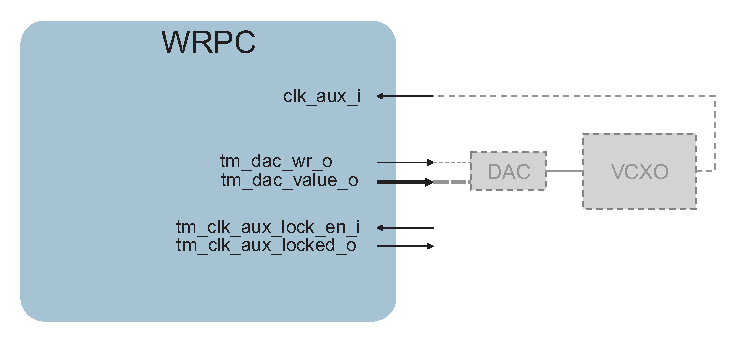
\includegraphics[width=.8\textwidth]{fig/adv_wrpc_clk.pdf}
    \caption{Aux clock synchronization interface}
  \end{center}
\end{figure}

The WRPC can syntonize auxiliary clock signals to the White Rabbit timebase. It
is done with a similar PLL that is used to discipline the local reference clock
(section \ref{basic:clk_rst}). WRPC provides tuning values for the VCXO producing
clock signal which is connected to \emph{clk\_aux\_i}.

\begin{center}
  \begin{tabular}{|l|l|p{9cm}|}
    \hline
    \multicolumn{3}{|l|}{\bf Signals description:}\\
    {\bf name} & {\bf size} & {\bf description} \\
    \hline \hline
    \texttt{clk\_aux\_i} & g\_aux\_clks & [optional] vector of auxiliary
    clocks that will be disciplined to WR timebase\\
    \hline
    \texttt{tm\_dac\_value\_o} & 24 & DAC value for tuning auxiliary clock
    (\emph{clk\_aux\_i})\\
    \texttt{tm\_dac\_wr\_o} & 1 & validates auxiliary DAC value\\
    \texttt{tm\_clk\_aux\_lock\_en\_i} & 1 & enable locking auxiliary clock to
    internal WR clock\\
    \texttt{tm\_clk\_aux\_locked\_o} & 1 & auxiliary clock locked to internal WR
    clock\\
    \hline
  \end{tabular}
\end{center}
